Image Metrics are Algorithms designed to evaluate quantitatively the similarity
between two images.


Image Metrics were introduced as components of the Registration Framework but
they can have other uses outside this framework.


Metrics Currently Available in ITK

\begin{itemize}
\item Mean Squares
\item Normalized Correlation
\item Mutual Information
\item Pattern Intensity
\end{itemize}

\subsection{Mean Squares}


Computes pixel-wise differences and sum their squares.

\begin{equation}
MS(A,B) = \frac{1}{N} \sum_i^N \left( A_i - B_i \right)^2
\end{equation}

\begin{center}
$A_i$ is the i-th pixel of Image A 
$B_i$ is the i-th pixel of Image B
$N$ is the number of pixels considered
\end{center}

The sum is computed over a restricted region
The optimal value is  Zero
Poor matches are large values 


Advantages

\begin{itemize}
\item Convenient for mathematical analysis 
\item Simplicity
\item Large capture radius
\end{itemize}

Disadvantages
\begin{itemize}
\item Limited to same image modality
\item Linear changes in intensity result in poor matching values
\end{itemize}


Computes pixel-wise cross-correlation and normalize it
by the square root of the autocorrelation of the images.

\begin{equation}
NC(A,B) = \frac{ \sum_i^N \left( A_i \cdot B_i \right) }
         { \sqrt { \sum_i^N A_i^2  \cdot \sum_i^N B_i^2 } }
\end{equation}


\begin{center}
$A_i$ is the i-th pixel of Image A\\ 
$B_i$ is the i-th pixel of Image B\\
$N$ is the number of pixels considered
\end{center}

The sum is computed over a restricted region
The optimal value is  One
Poor matches are small values 


\subsection{Normalized Correlation}


Advantages

\begin{itemize}
\item Insensitive to multiplicative factors
\item Profile is more pointy (high precision)
\end{itemize}

Disadvantages
\begin{itemize}
\item Limited to same image modality
\item Reduced capture radius
\end{itemize}


\subsection{Pattern Intensity}

Computes pixel-wise differences and add them after passing them through a
bell-shaped function $\frac{1}{1+x^2}$

\begin{equation}
PI(A,B) =  \sum_i^N \frac{ 1 }{ 1 + \lambda \left( A_i - B_i \right) ^ 2 }
\end{equation}

\begin{center}
$A_i$ is the i-th pixel of Image A 
$B_i$ is the i-th pixel of Image B
$N$ is the number of pixels considered
$\lambda$ controls the capture radius
\end{center}

The sum is computed over a restricted region
The  Optimal value is $N$
Poor matches are small values 


\subsection{Pattern Intensity}

Advantages

\begin{itemize}
\item Produce poor values when few pixels are considered
\item Capture radius can be controled
\item Profile is very pointy (high precision)
\end{itemize}

Disadvantages
\begin{itemize}
\item Limited to same image modality
\item Its derivative is high at the peak this is a problem for some optimizers
\item Sensitive to linear changes in intensity
\end{itemize}


\subsection{Mutual Information}


Computes how much uncertainty about one image can be
reduced by having the information contained in the other
image.

Information == Reduction in uncertainty

\begin{equation}
H(A)=-\sum _{i=1}^{G}p(a_{i})\cdot \log p(a_{i})
\end{equation}

\begin{center}
$a_{i}$ is the i-th gray level of image A
$G$ is the number of gray levels in image A
$p(a_{i})$ is the probability of finding $a_{i}$ in a pixel of A
\end{center}

\begin{equation}
H(A) = \mbox{Entropy of} A
\end{equation}

$p(a_{i})$ values can be estimated from the image histogram.

A population of pixel pairs can be obtained by taking homologous pixels from
two images.

Joint Entropy can be computed from the statistical distribution of gray levels.

\begin{equation}
H(A,B)=-\sum _{i=1}^{G_{A}}\sum _{j=1}^{G_{B}}p\left( a_{i},b_{j}\right) \cdot \log p\left( a_{i},b_{j}\right)
\end{equation}


\begin{center}
$a_{i}$ is the i-th gray level of image A
$b_{j}$ is the j-th gray level of image B $p\left( a_{i},b_{j}\right)$ is the
probability of finding the gray level $a_{i}$ associated with the gray level
$b_{j}$ in the same pair of pixels.
\end{center}


If the gray levels of A are independent of B

\begin{equation}
p\left( a_{i},b_{j}\right) =p\left( a_{i}\right) \cdot p\left( b_{j}\right) 
\end{equation}


and then 

\begin{equation}
H(A,B)=H(A)+H(B)
\end{equation}


but if there is any dependency

\begin{equation}
H(A,B)<H(A)+H(B)
\end{equation}


the difference is called Mutual Information : \( I(A,B) \)

\begin{equation}
I(A,B)=H(A)+H(B)-H(A,B)
\end{equation}



\subsubsection{Parzen Windowing}

The probability distributions of gray levels are in general unkown.

They can be estimated by taking samples (pixels) from the image and
reconstructing a continuous function by convolving the samples with a smoothing
kernel function.

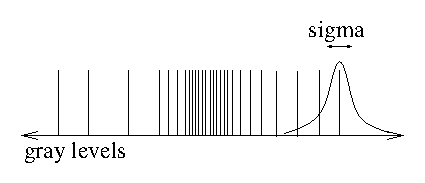
\includegraphics{ParzenWindowing1.eps}

This is typically done with a Gaussian. A value of sigma should be selected
somehow related with the number of pixels sampled.  

\subsubsection{Convolution with the
smoothing function}

\resizebox*{0.5\columnwidth}{!}{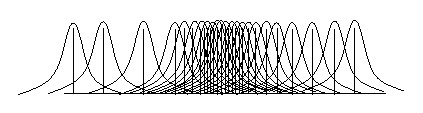
\includegraphics{ParzenWindowing2.eps}}

Resulting continuous probability distribution 

\resizebox*{0.5\columnwidth}{!}{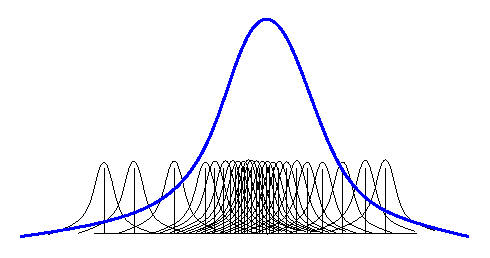
\includegraphics{ParzenWindowing3.eps}}


Advantages

\begin{itemize}
\item Allows to compare different image modalities
\item Few samples (pixels) are required
\end{itemize}

Disadvantages

\begin{itemize}
\item Requires to tune parameters (number of samples and parzen windowing probability distributions estimation)
\item Not suitable for images related by linear relationships
\end{itemize}





